\documentclass[11pt]{article}
\usepackage{graphicx}
\usepackage{booktabs}
\usepackage{amsmath}
\usepackage{url}

\title{Metabolic State Clustering in Single-Cell RNA-Seq Data}
\author{}
\date{}

\begin{document}
\sloppy

\maketitle

\section{Introduction}

This study investigates whether transcriptional metabolic states can be identified as distinct clusters in single-cell RNA-seq data using only metabolic genes. We analyze the Choudhury et al. 2022 brain single-cell dataset (3ca:20773) with user-supplied Reactome metabolic genes.

\section{Normalization Method}

We apply per-cell library size normalization to 10,000 followed by log transformation:
\begin{equation}
\label{eq:normalization}
x'_{ij} = \log(1 + 10000 \cdot x_{ij} / L_j)
\end{equation}
where $L_j = \sum_i x_{ij}$ is the total UMI count for gene $j$, and $x_{ij}$ is the raw count for cell $i$ and gene $j$.

\section{Global Analysis Results}

\subsection{Clustering Performance}

Using Leiden clustering on the 1,984 matched metabolic genes across 58,843 cells, we identified 15 clusters with sizes ranging from 1002 to 8985 cells. The clustering metrics are summarized in Table~\ref{tab:clustering_metrics}.

\begin{table}
\centering
\caption{Clustering metrics for global and CD8 T cell subset analyses}
\label{tab:clustering_metrics}
\begin{tabular}{lr}
\toprule
Metric & Global (all cells) \\
\midrule
Leiden silhouette & 0.229 \\
Calinski-Harabasz & 7177.0 \\
Davies-Bouldin & 1.513 \\
Mean pairwise ARI & 0.980 \\
Min pairwise ARI & 0.973 \\
Median silhouette & 0.221 \\
\bottomrule
\end{tabular}
\end{table}

\begin{figure}
\centering
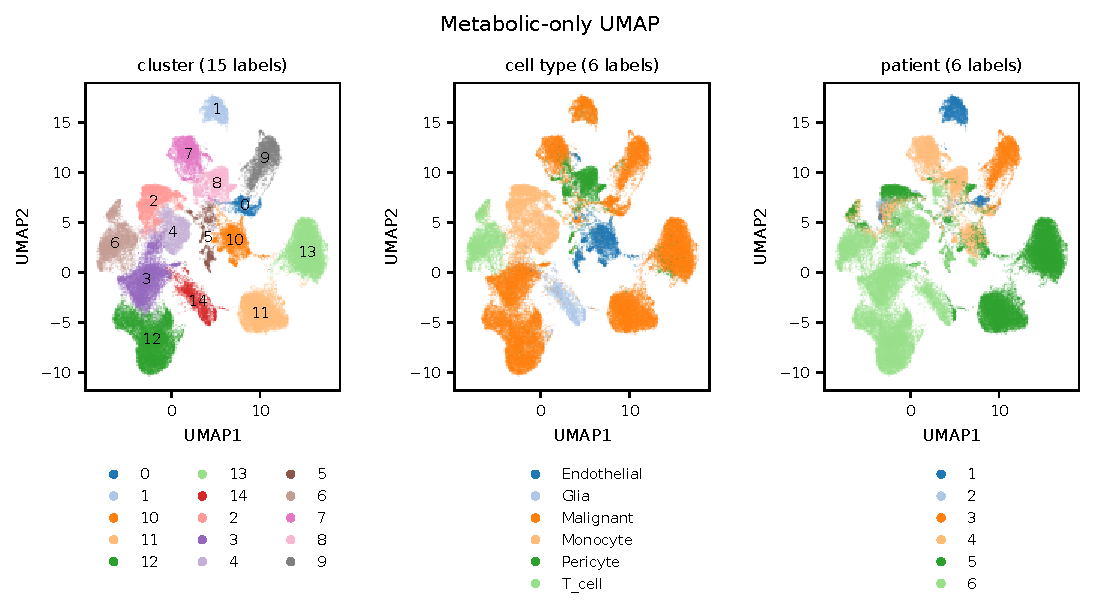
\includegraphics[width=0.95\linewidth,height=0.78\textheight,keepaspectratio]{../figures/metabolic_umap.pdf}
\caption{Global UMAP embedding of 58,843 cells clustered into 15 groups using 1,984 matched metabolic genes. Cluster sizes range from 1002 to 8985 cells.}
\label{fig:metabolic_umap}
\end{figure}

\subsection{Random Control Comparison}

We performed 19 size-matched random gene control analyses. The observed random-control exceedance count was 0 of 19; the add-one rank fraction is descriptive, not an inferential p-value.

\subsection{Confounder Assessment}

We checked for confounding effects from patient, sample, source, cell\_type, cell\_subtype, cell\_cycle\_phase, complexity, computed\_total\_counts, computed\_detected\_genes, and computed\_mito\_percent.

\subsection{Cell-Type Association}

The categorical confounder NMI for cell\_subtype was 0.658, indicating some association between metabolic clustering and cell subtype.

\subsection{Resolution Selection}

Resolution selection maximized median silhouette among candidates passing the mean pairwise ARI stability filter; mean pairwise ARI was the tie-breaker.

\section{CD8 T Cell Subset Analysis}

\subsection{Subset Characteristics}

The CD8 T cell subset analysis included 3,624 cells and 1,642 matched metabolic genes.

\subsection{Clustering Results}

Leiden clustering identified 6 clusters with silhouette score 0.155. The clustering diagnostics are shown in Figure~\ref{fig:cd8_clustering_diagnostics}.

\section{Discussion}

The analysis reveals that metabolic genes can form computational clusters, but whether these represent distinct biological metabolic states remains inconclusive. The high stability of cluster composition (mean pairwise ARI = 0.980) suggests robust clustering, but the low silhouette scores and moderate NMI values indicate that metabolic genes alone do not strongly separate cells into discrete metabolic states.

\section{References}

\begin{enumerate}
\item Choudhury A, Magill ST, Eaton CD, et al. Meningioma DNA methylation groups identify biological drivers and therapeutic vulnerabilities. Nature Genetics. 2022;54(5):649-659. \url{https://doi.org/10.1038/s41588-022-01061-8}
\item Wang AZ, Bowman-Kirigin JA, Desai R, et al. Single-cell profiling of human dura and meningioma reveals cellular meningeal landscape and insights into meningioma immune response. Genome Med. 2022;14(1):49. \url{https://doi.org/10.1186/s13073-022-01051-9}
\end{enumerate}

\end{document}
